\let\negmedspace\undefined
\let\negthickspace\undefined
\documentclass[journal]{IEEEtran}
\usepackage[a5paper, margin=10mm, onecolumn]{geometry}
%\usepackage{lmodern} % Ensure lmodern is loaded for pdflatex
\usepackage{tfrupee} % Include tfrupee package

\setlength{\headheight}{1cm} % Set the height of the header box
\setlength{\headsep}{0mm}     % Set the distance between the header box and the top of the text

\usepackage{gvv-book}
\usepackage{gvv}
\usepackage{cite}
\usepackage{amsmath,amssymb,amsfonts,amsthm}
\usepackage{algorithmic}
\usepackage{graphicx}
\usepackage{textcomp}
\usepackage{xcolor}
\usepackage{txfonts}
\usepackage{listings}
\usepackage{enumitem}
\usepackage{mathtools}
\usepackage{gensymb}
\usepackage{comment}
\usepackage[breaklinks=true]{hyperref}
\usepackage{tkz-euclide} 
\usepackage{listings}
% \usepackage{gvv}                                        
\def\inputGnumericTable{}                                 
\usepackage[latin1]{inputenc}                                
\usepackage{color}                                            
\usepackage{array}                                            
\usepackage{longtable}                                       
\usepackage{calc}                                             
\usepackage{multirow}                                         
\usepackage{hhline}                                           
\usepackage{ifthen}                                           
\usepackage{lscape}
\usepackage{circuitikz}
\tikzstyle{block} = [rectangle, draw, fill=blue!20, 
    text width=4em, text centered, rounded corners, minimum height=3em]
\tikzstyle{sum} = [draw, fill=blue!10, circle, minimum size=1cm, node distance=1.5cm]
\tikzstyle{input} = [coordinate]
\tikzstyle{output} = [coordinate]


\begin{document}

\bibliographystyle{IEEEtran}
\vspace{3cm}

\title{8.6-6.5-1.1}
\author{EE24BTECH11063 - Y. Harsha Vardhan Reddy}
 \maketitle
% \newpage
% \bigskip
{\let\newpage\relax\maketitle}

\renewcommand{\thefigure}{\theenumi}
\renewcommand{\thetable}{\theenumi}
\setlength{\intextsep}{10pt} % Space between text and floats


\numberwithin{equation}{enumi}
\numberwithin{figure}{enumi}
\renewcommand{\thetable}{\theenumi}

\textbf{Question}:\\
Find the minimum value of the function\\
$$f(x)=\brak{2x-1}^2+3$$\\
\solution \\
\\
\textbf{Theoritical solution:}\\
Given,\\
\begin{align}
    \frac{dy}{dx}=4\brak{2x-1}=0\\
    \implies x=\frac{1}{2}\\
    \frac{d^2y}{dx^2}=8\\
\end{align}
Since, $\frac{d^2y}{dx^2}>0$, at $x=\frac{1}{2}$ there exists minimum  \\
Therefore, $f\brak{\frac{1}{2}}=3$ is the minimum value of the function\\
\textbf{Computational Solution Using Gradient Descent} \\
To verify the analytical results, we use gradient descent to find the local minimum \\
Gradient Descent for local minimum : \\ 
 - Start with $x_0 = 4$ \\
 - Update $x$ iteratively using 
\begin{align}
    x_{n+1} = x_n - \eta \cdot f'(x_n)
\end{align}
where :
\begin{align}
    \eta = 0.1 
\end{align}
\begin{align}
    f'(x) = 4(2x-1) 
\end{align}
\begin{align}
    x_{n+1} = x_n - \eta \cdot (4(2x_n-1))
\end{align}
\textbf{Computational Results} \\
 - Local minimum 
 \begin{align}
     x \approx 0.5,\text{ } g(x) \approx 3.000
 \end{align} 
 \begin{figure}[ht!]
   \centering
   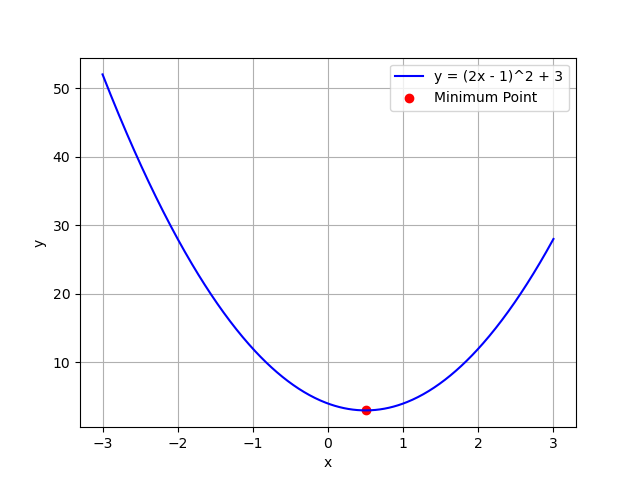
\includegraphics[width=\columnwidth]{figs/Figure_1.png}
\end{figure}
\end{document}
